\documentclass[a4paper]{jpconf}
\usepackage{graphicx}
\begin{document}
\title{Performance of Prototype of Optically Readout TPC with a $^{55}$Fe source}

\author{
{I.~Abritta~Costa}$^{a}$,
{E.~Baracchini}$^{b}$,
{F.~Bellini}$^{a,c}$,
{L.~Benussi}$^{d}$,
{S.~Bianco}$^{d}$,
{G.~Cavoto}$^{a,c}$,
{E.~Di~Marco}$^{a}$,
{G.~Maccarrone}$^{d}$,
{M.~Marafini}$^{e}$,
{G.~Mazzitelli}$^{d}$,
{A.~Messina}$^{a,c}$,
{D.~Piccolo}$^{d}$,
{D.~Pinci}$^{a}$,
{F.~Renga}$^{a}$,
{F.~Rosatelli}$^{d}$ and
{S.~Tomassini}$^{d}$
\\
\address{$^a$ Istituto~Nazionale~di~Fisica~Nucleare,  
 Sezione di Roma, I-00185, Italy}
\address{$^b$ Gran~Sasso~Science~Institute~L'Aquila, I-67100, Italy}
\address{$^c$ Dipartimento di Fisica, Sapienza Universit\`a di Roma, I-00185, Italy} 
\address{$^d$ Istituto Nazionale di Fisica Nucleare,  Laboratori Nazionali di Frascati, I-00040, Italy}
\address{$^e$ Museo Storico della Fisica e Centro Studi e Ricerche "Enrico Fermi", Piazza del Viminale 1, Roma, I-00184, Italy}
}

\ead{emanuele.dimarco@roma1.infn.it}

\begin{abstract}
The performances of an optical readout of Time Projection Chambers
(TPCs) with multiple Gas Electron Multipliers (GEMs) amplification
stages are presented.  The detector is characterized by using a
$^{55}$Fe source within a 7 litre sensitive volume detector in
different electric field configurations.  This prototype is developed
as a part of the R\&D for the CYGNO project for an application to
direct Dark Matter search through the detection of tracks of nuclear
recoils in the gas within the keV energy range.
\end{abstract}

\section{Experimental setup and data analysis}
\label{sec:daq}

All measurements described in this work were carried out on a prototype for the future CYGNO experiment, called Large Elliptical MOdule (LEMON, Fig. \ref{fig:lemon})
which is described in details in refs. \cite{bib:eps, bib:ieee17, bib:ieee18}.

\begin{figure}[htbp]
\centering
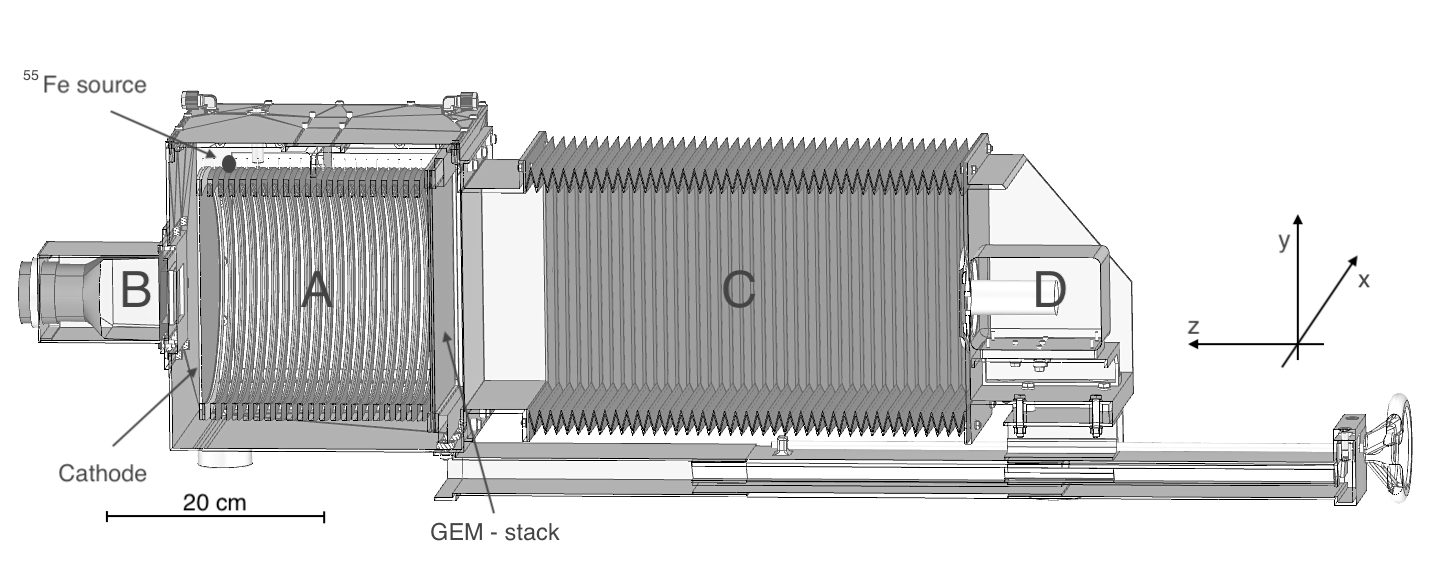
\includegraphics[width=.85\textwidth]{sex_bw-2.png}
\caption{Drawing of the experimental setup.
In particular, the elliptical field cage close on one side by the triple-GEM structure and on the other 
side by the semitransparent cathode (A), 
the PMT (B), 
the adaptable bellow (C) and the CMOS camera with its lens (D) 
are visible.}
\label{fig:lemon}
\end{figure}

The main elements of LEMON are:
\begin{itemize}
    \item A sensitive volume (A) filled with 7 litre of He/CF$_4$ 60/40 gas mixture at atmospheric pressure, surrounded by a field cage (FC) composed of 20 elliptic silver plated wire rings with axes of 24 cm (along {\it x}) and 20 cm (along {\it y}) and a depth of 20 cm (along {\it z});
    \item The sensitive volume is closed on one side by a semi-transparent cathode made of a thin wire mesh and on the other side by a structure of three 20$\times$24 cm$^2$, 50~$\mu$m thick GEMs;
    \item The whole structure is contained in a gas-tight box with two
      transparent windows on the cathode and the GEM sides;
    \item On the cathode side, beyond the window, a fast photo-sensor
      PMT
      %\footnote{Photonics XP3392, 5 ns rise-time, 76mm square-window}
      (B) is placed to readout all the light produced by the GEMs;
    \item On the other side, downstream to an adjustable bellow (C),
      an ORCA Flash 4.0 camera,
      % \footnote{For more details visit www.hamamatsu.com} based on a
      1.33~$\times$~1.33~cm$^2$ scientific CMOS sensor (subdivided in
      2048~$\times$~2048 pixels with an active area of
      6.5~$\times$~6.5~$\mu$m$^2$ each) and equipped with a Schneider
      lens
      %\footnote{25 mm focal length, 0.95 aperture} (D) is placed at a
      distance of 52.5~cm (i.e. 21 Focal Length, FL) for the
      acquisition of the light produced in the GEM holes. In this
      configuration, the sensor faces a surface of
      $26~\times~26$~cm$^2$ and therefore each pixel at an area of
      $130 \times 130~\mu$m$^2$. The geometrical acceptance $\Omega$
      therefore results to be $1.6 \times 10^{-4}$
      \cite{bib:ieee_orange}.
\end{itemize}

A $^{55}$Fe source, with an activity of about 100 Bq, was placed
between two FC rings, 18 cm far from the GEM as shown in
Fig. \ref{fig:lemon}.  Because of the short distance between the
plastic rings supporting the FC wires and their width along the {\it
  x} and {\it y} directions, these acted as a collimator for the
photons emitted by the source, so that the effective distance from the
GEMs of their interactions with the gas molecules was estimated to be
18~$\pm$~2 cm. Electrons produced within the sensitive volume are
drifted by the electric field (E$_{\rm d}$) present within the FC,
toward the GEMs where the multiplication process takes place. Typical
operating conditions of the detector are: E$_{\rm d}$~=~600~V/cm, an
electric field in the GEM produced by V$_{\rm GEM}$~=~460V for each
GEM plane and a transfer field E$_{\rm t}$~=~2~kV/cm. The maximum
value of (E$_{\rm d}$) is limited by the maximum voltage provided by
the HV generator (15 kV) used for the measurements reported in this
paper.

The results presented in this poster are based on data 
acquired by the ORCA sensor 
in free running mode, without any trigger. The light produced during the multiplication processes in the GEM were recorded with an exposure of 100 ms.
The analysis algorithm is based on two steps:
\begin{enumerate}
    \item {\it Pedestal subtraction}. A {\it blind run} of 100 images
      was acquired with the sensor in total dark. For each pixel, the
      pedestal is evaluated as the average number of counts recorded
      in this run and is subtracted to the counts collected in all
      recorded images. A sensor noise of 1.9 photons per pixel was
      measured as rms of the pedestal distribution.
    \item {\it Clustering}: a very simple nearest neighbor-cluster
      (NNC) clustering algorithm was developed. A lower resolution
      version of each image was created with {\it macro-pixels} made
      by matrices of 4$\times$4 pixels.  The average count over the 16
      pixels, after subtracting their pedestal values, is assigned to
      each macro-pixel.  A cluster is reconstructed by at least two
      neighbouring macro-pixels having more than 2 counts (i.e. 2
      photons \cite{bib:jinst_orange1}) each.
\end{enumerate}

Figure~\ref{fig:spot} shows an example of an image of two light 
spots due the interaction of the $^{55}$Fe photons in the gas.

\begin{figure}[htbp]
\centering
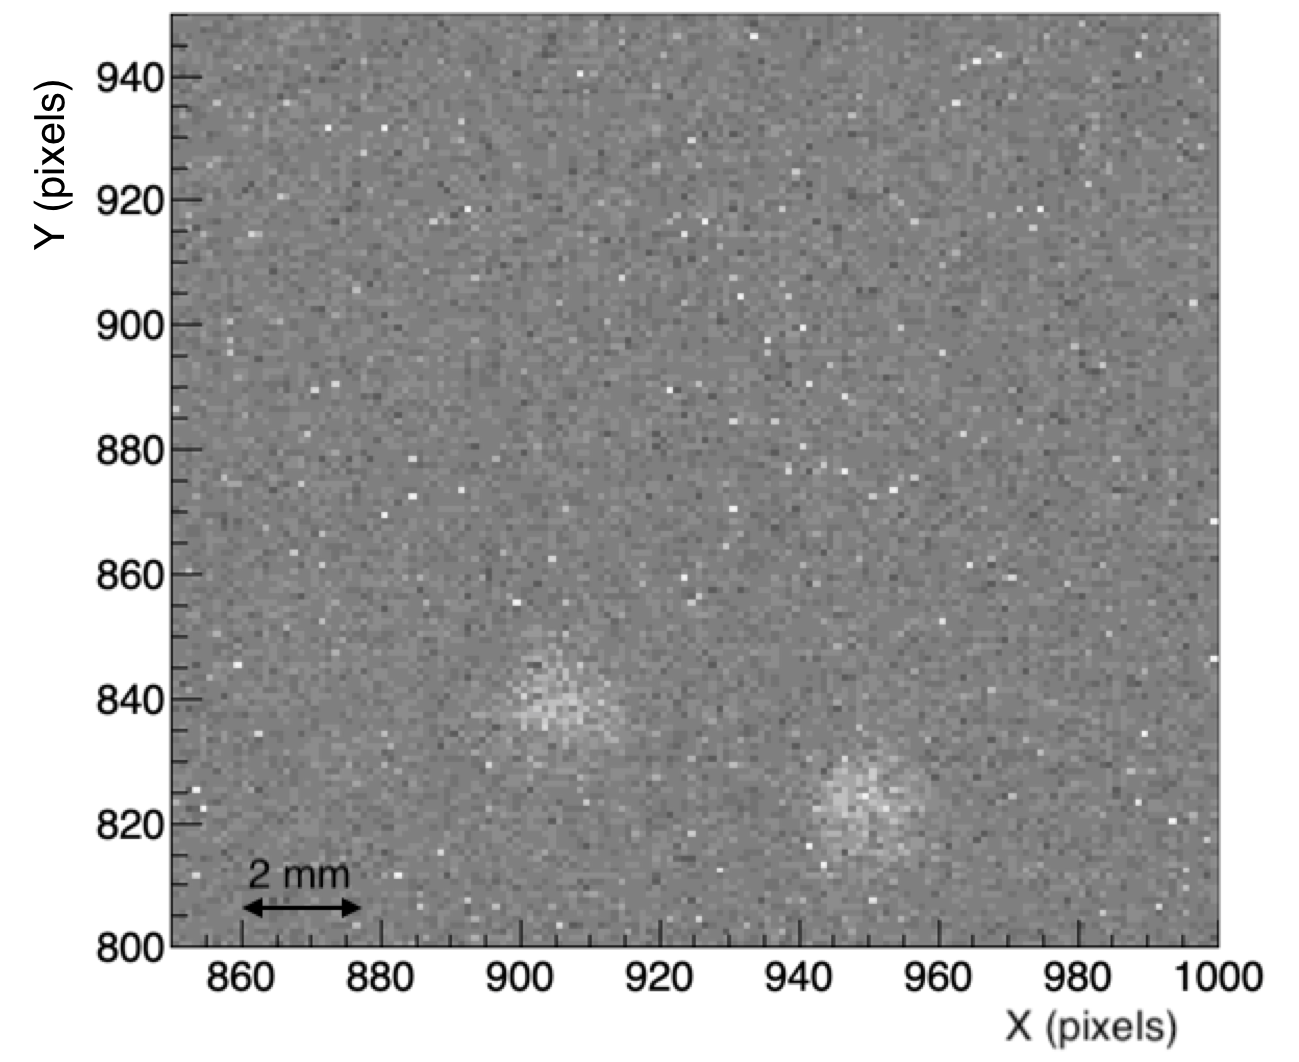
\includegraphics[width=.45\textwidth]{spot_xRay_841.png}
\caption{Example of two clusters due to X-ray interaction in gas.}
\label{fig:spot}
\end{figure}

\section{Backgrounds}
\label{sec:bkg}

The CMOS sensor used for the measurements has two main sources of noise: 
\begin{itemize}
    \item a dark current of about 0.06 electrons per second per pixel;
    \item a readout noise of about 1.4 electrons rms (in our set-up it
      was found to be slightly larger probably due to an effect of
      {\it ageing} of the sensor built more than 5 years ago);
\end{itemize}

The sensor electronic noise represents a possible unavoidable
instrumental background and it can generate {\it ghost-clusters}.  The
distribution of the light in each {\it ghost-cluster} found in the
{\it blind run} is shown in Fig.~\ref{fig:hq_ghost} (left).

The shape of the distribution is determined by the positively-definite
counts of photons in the cluster. Its shape is used to estimate an
operative threshold that allows to suppress fake signals due to sensor
noise. The distribution is fitted with an exponential function and the
tail extrapolated with this function.  From the fitted parameters, and
by taking into account that a run lasts 10 s, it is possible to
extrapolate the probability of having a {\it ghost-clusters} with an
amount of light larger than a given threshold. As an example, a
threshold of 300 photon counts corresponds to 1$\times$10$^{-4}$ {\it
  ghost-clusters}/second.

The GEM structure can, in principle, create a diffused light
background because of possible micro-discharges.  To evaluate it, the
distribution of the light in the clusters reconstructed outside the
sensitive area was studied.  As it is shown in Fig.~\ref{fig:hq_ghost}
(right), the obtained distribution is similar to the one due to the
sensor electronic noise and has a tail that can be described with an
exponential with a slope which is very similar to the one obtained for
the sensor noise.
%
\begin{figure}[htbp]
\centering
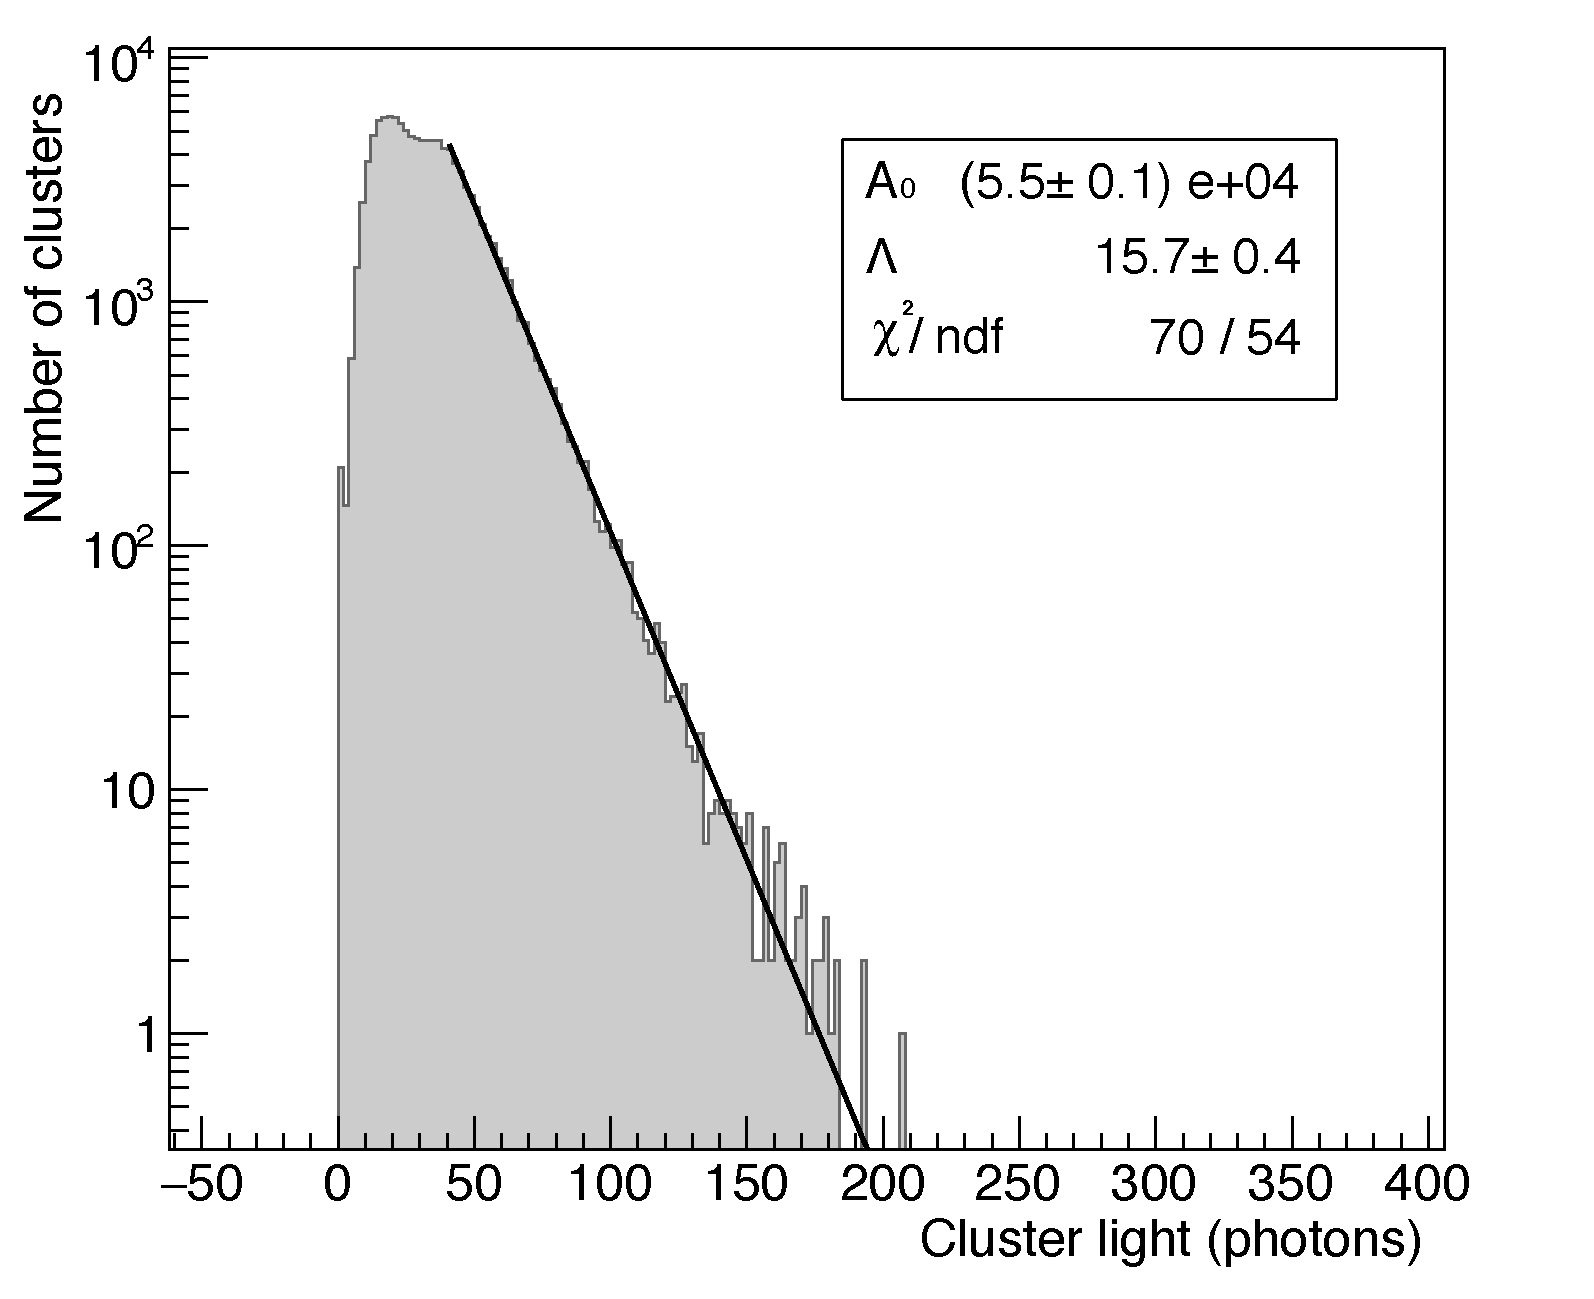
\includegraphics[width=.40\textwidth]{hq_run818.pdf}
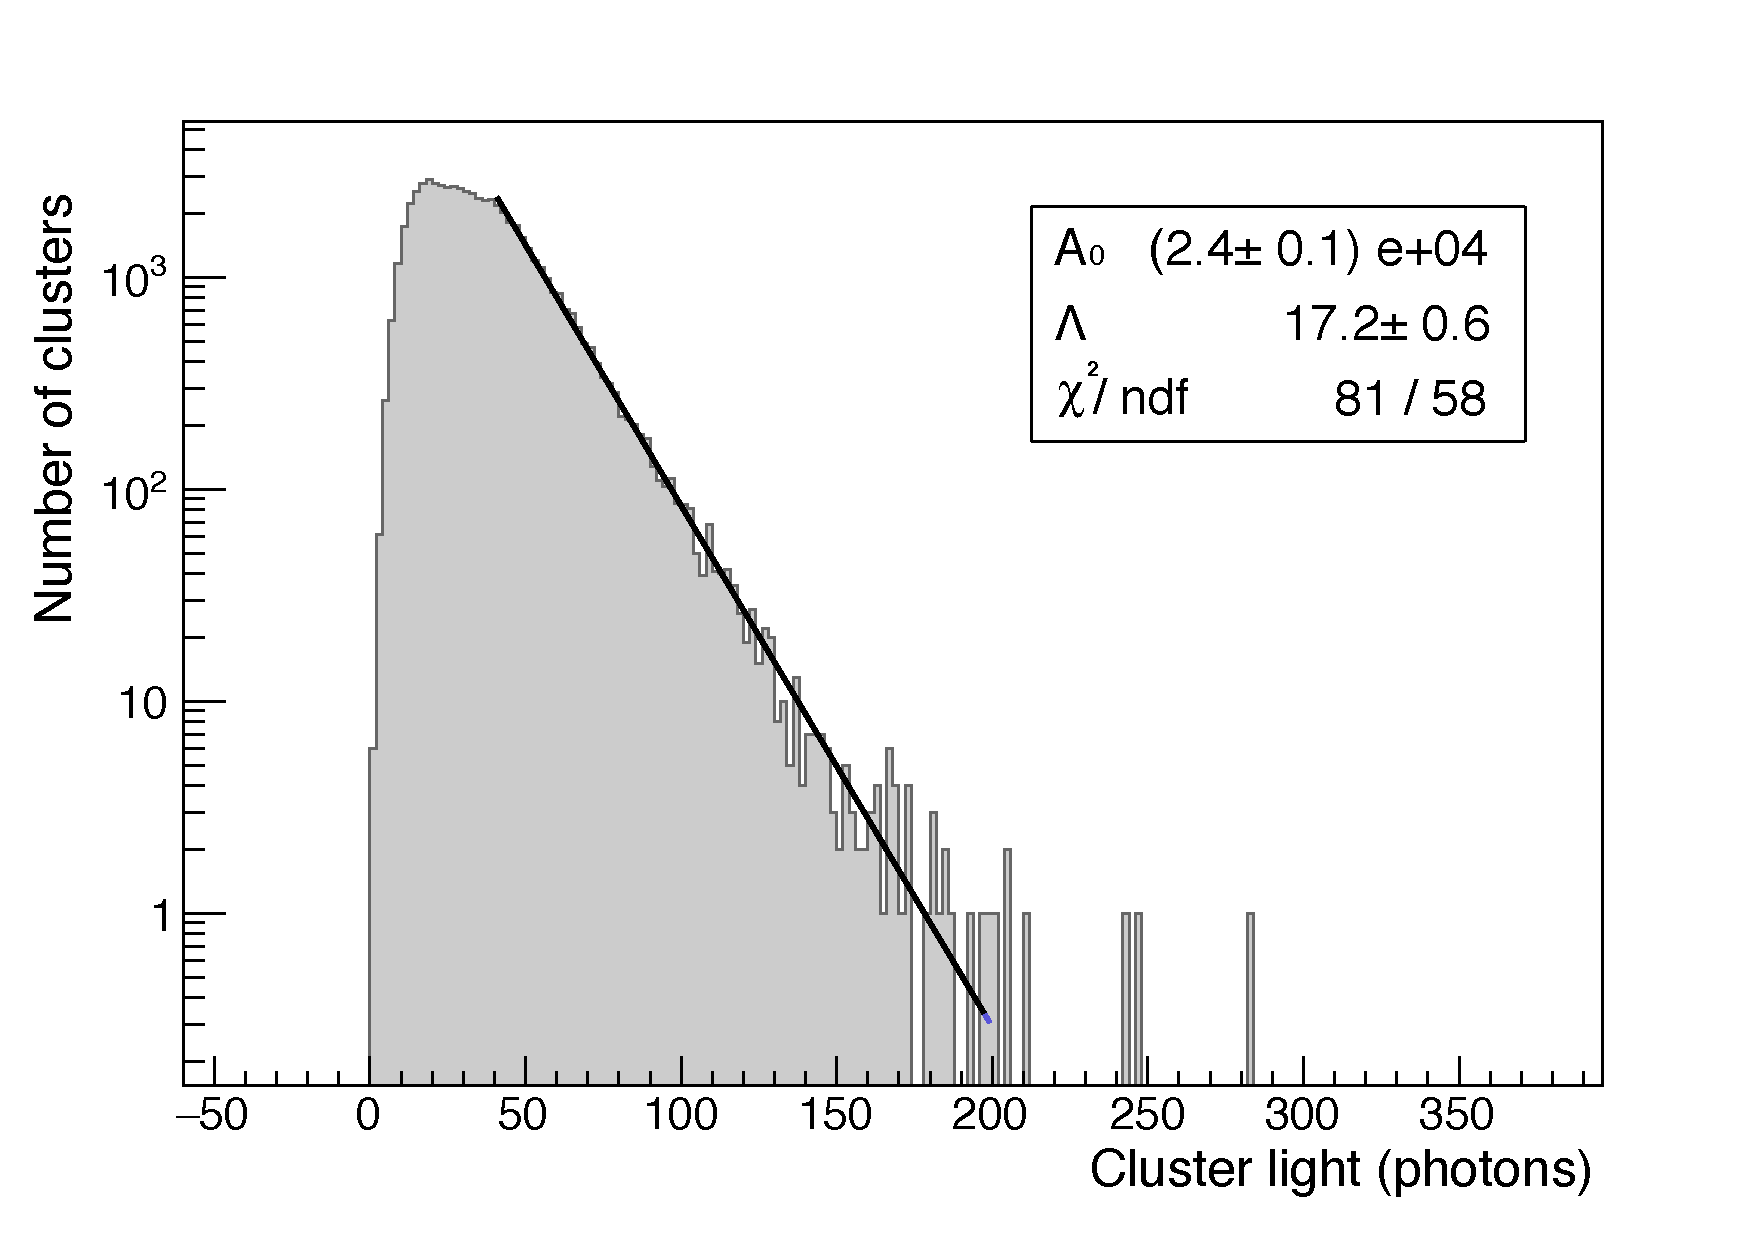
\includegraphics[width=.40\textwidth,height=.35\textwidth]{hqOut_run823.pdf}
\caption{Left: Distribution of the light in clusters reconstructed in
  a run with blind sensor.  Right: distribution of the light recorded
  clusters reconstructed outside from the sensitive area in a run with
  $^{55}$Fe source with superimposed exponential
  fit. \label{fig:hq_ghost}}
\end{figure}
%
The few events found outside the bulk of the distribution are short
tracks very likely due to events occurred close to the GEM, where the
residual electric field of the GEM is able to capture electrons and
drive them toward the multiplication channels.

As already described in Sec.~\ref{sec:daq}, within the FC area an
evident diffused and flat background is visible.  To study it, a run
without the radioactive source was acquired. Superimposing the images
of all the reconstructed clusters in the whole run, results into an
observed spatial distribution of clusters similar to the one found in
presence of the source.

Figure~\ref{fig:bkg_evt} shows 10 overlapped events randomly chosen within the run.
%
\begin{figure}[htbp]
\centering
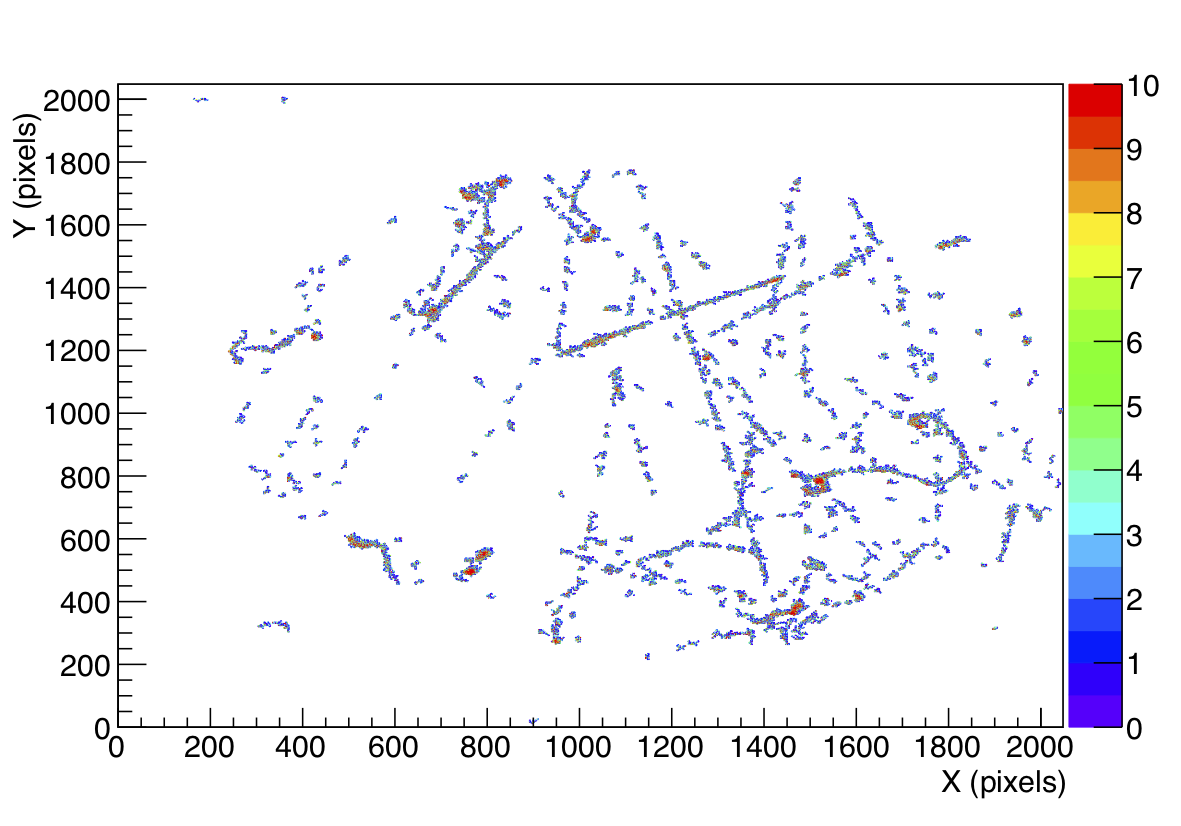
\includegraphics[width=.55\textwidth]{hDisplay_run121.png}
\caption{Example of 10 events acquired in a run without the $^{55}$Fe source within the detectors. Color scale indicates the number of photons collected per pixel.}
\label{fig:bkg_evt}
\end{figure}
%
They appear as to be mostly tracks due to cosmic rays or low energy
electrons from natural radioactivity.  In a radio-pure apparatus
operating underground such a background is expected to be strongly
suppressed.  Moreover, pattern recognition should be able to identify
and reject residual events. For this reason, the effect of this
background is not taken into account in this paper for the evaluation
of the possible operative threshold.


\section{Cluster size and light spectrum}

For each run, the spectrum of the total light in clusters reconstructed within the sensitive area and the distribution of their size (i.e. the number of over-threshold pixels) are studied.
Figure \ref{fig:spectra} shows an example of these distributions for a run taken with V$_{\rm GEM}$~=~450 V, E$_{\rm d}$ = 600~V/cm and E$_{\rm t}$ = 2~kV/cm.

\begin{figure}[htbp]
\centering
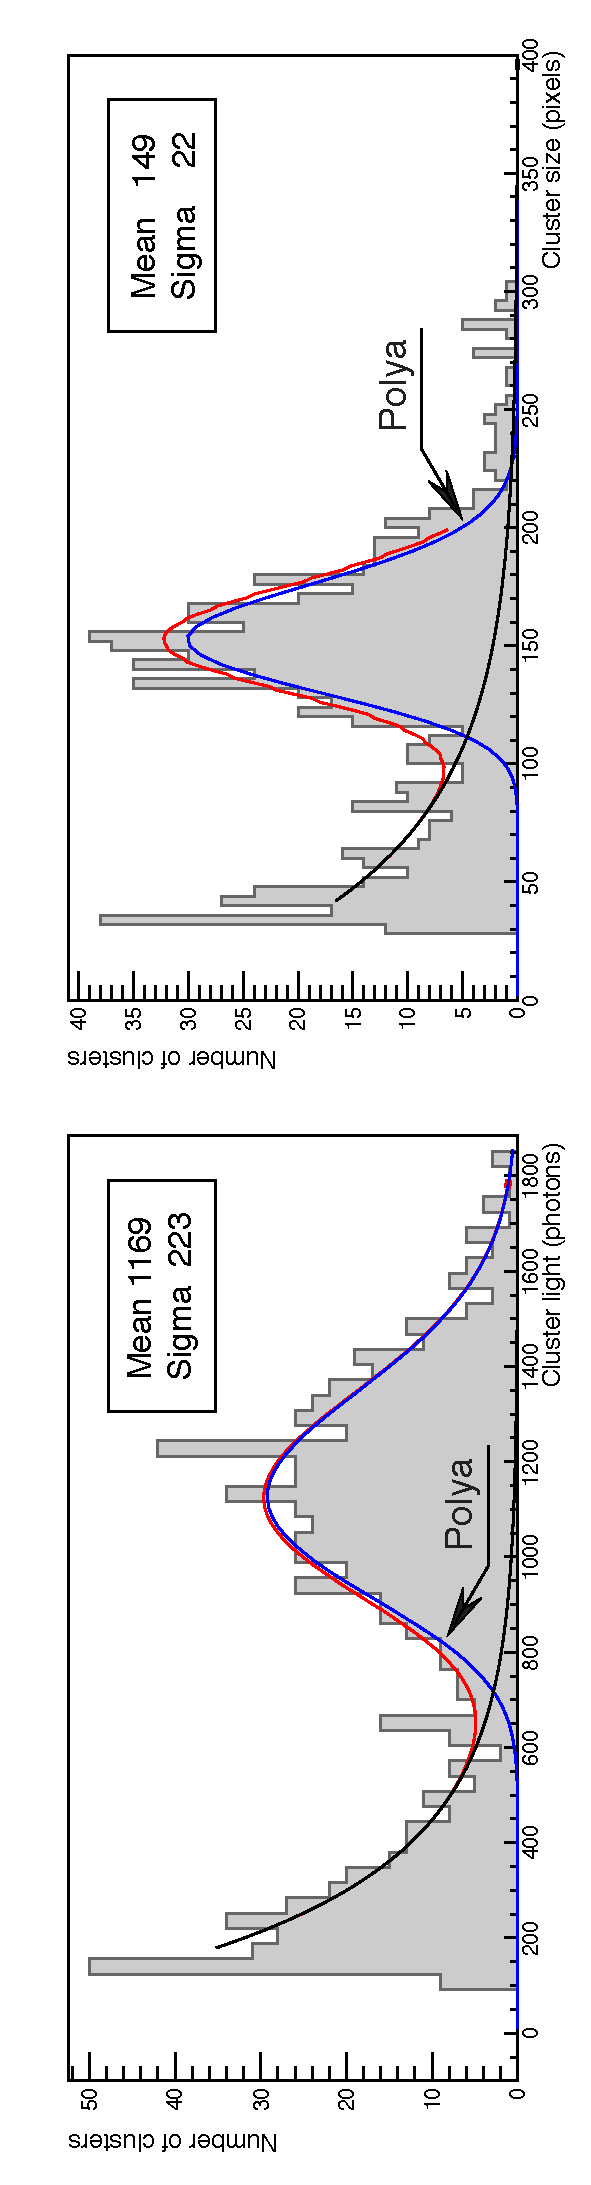
\includegraphics[width=.27\textwidth, angle=270]{hq_s_Xray_run823.pdf}
\caption{Distribution of total light (left) and number of illuminated pixels (right) for a run taken with V$_{\rm GEM}$~=~450 V, E$_{\rm d}$~=~600 V/cm and E$_{\rm t}$~=~2 kV/cm.}
\label{fig:spectra}
\end{figure}

Only clusters with at least 30 pixels over-threshold were
considered. The distribution is fitted with the sum of an exponential
function to model the background due to natural radioactivity
(Sec.~\ref{sec:bkg}), and a Polya function, expressed by
Eq.~\ref{fun:polya}, often used to describe the response spectrum of
MPGD \cite{bib:rolandiblum}:
%
\begin{equation}
   P(n)=\frac{1}{b\overline{n}}\frac{1}{k!}\left(\frac{n}{b\overline{n}}\right)^k \cdot e^{-n/b\overline{n}}
   %A\frac{\Gamma(r+k)}{k!\Gamma(r)} p^k (1-p)^r e^{(-x/\lambda)} 
\label{fun:polya}
\end{equation}
%
%where n represents the number of secondary electrons, 
where $b$ is a free parameter and $k=1/b-1$. The distribution has $\overline{n}$ as expected value, while the variance is governed by its mean and the parameter $b$: $\sigma^2=\overline{n}(1+b\overline{n})$. 
From the result of the fits it is possible to evaluate:
\begin{itemize}
\item the expected value of the distribution $\overline{n}$ and its
  variance $\sigma^2$. These parameters, when fitted on the light
  distributions, give the detector response in term of number of
  photons and the energy resolution. The latter will thus indicate the
  variance ($\sigma$) of the Polya fit in the whole paper.  When
  fitting the number of illuminated pixels distribution, the average
  size of the clusters can be evaluated by taking into account the
  effective area of $130~\times 130~\mu$m$^2$ (see
  Sect. \ref{sec:daq}) acquired by each single pixel.
\item the integral of the Polya component, that is proportional to the
  total number of reconstructed clusters and that can be used to
  evaluate the detection efficiency;
\end{itemize}
Since, as it is shown on the left of Fig.~\ref{fig:spectra}, in this
configuration 1169~$\pm$~223 photons are collected per cluster
(i.e. each 5.9~keV released), a threshold of 400 photons corresponds
to about 2~keV released in the sensitive volume.  The average cluster
size was found to be 149 pixels (Fig.~\ref{fig:spectra}, right).

\section{Results}
The response of the detector to the $^{55}$Fe source has been studied
as a function of three different operative parameters: V$_{\rm GEM}$,
E$_{\rm d}$ and E$_{\rm t}$.  The results are reported in the
following.

\begin{enumerate}
\item \textbf{Dependence on the voltage applied to the GEM (V$_{\rm GEM}$)}

The voltage applied to the GEM (V$_{\rm GEM}$) determines the gain and
therefore the light yield of the structure. Then, the average number
of collected photons per cluster and its fluctuations as a function of
V$_{\rm GEM}$ is expected to raise increasing V$_{\rm GEM}$.
Figure~\ref{fig:vgem1} (left) shows that the detector light yield
increases exponentially and doubles every V$_{\rm GEM} =$~30 V step.
The energy resolution is also found not to be significantly dependent
on the voltage applied to the GEM with a value around 20\%. Both
results are found in good agreement with results obtained with similar
experimental setup \cite{bib:loomba}.


\begin{figure}[htbp]
\centering
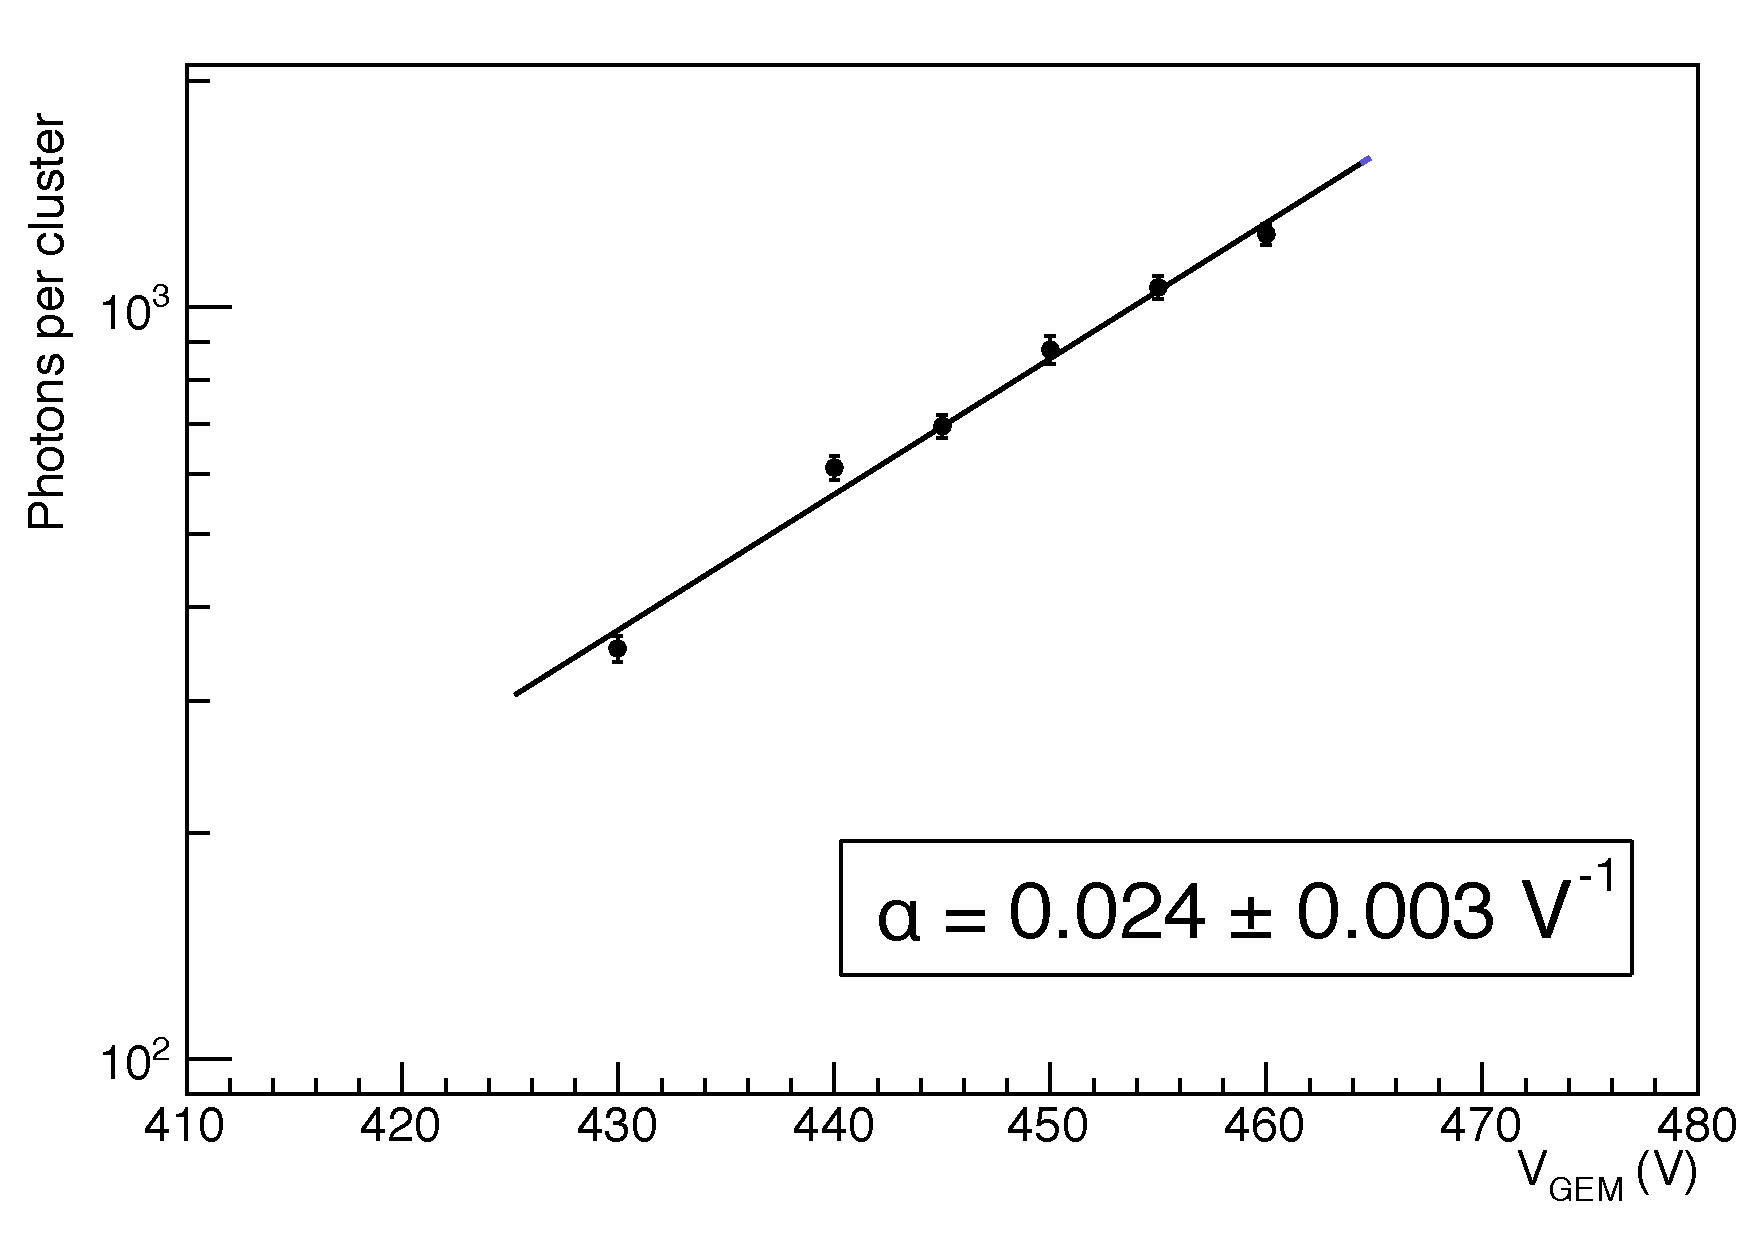
\includegraphics[width=.42\textwidth]{gPhotFar_Vg.pdf}
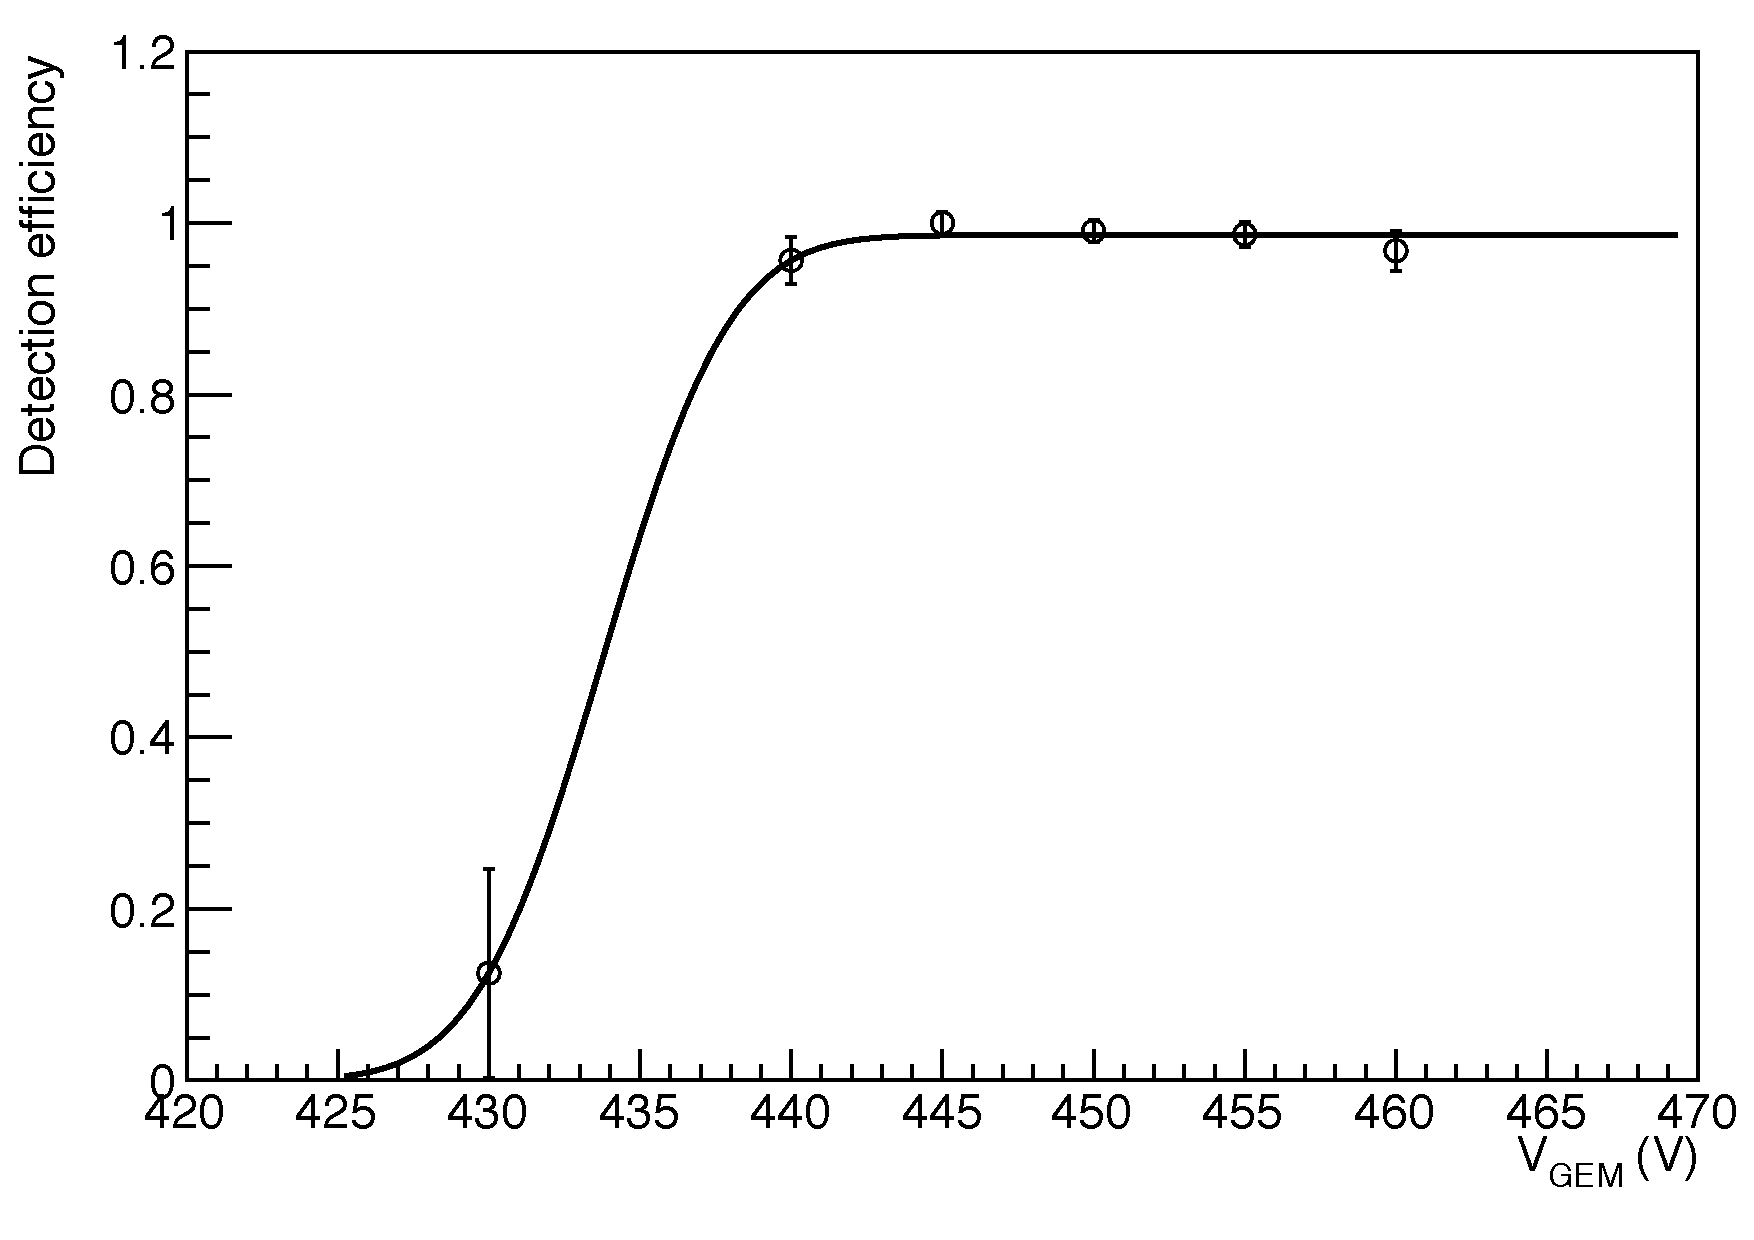
\includegraphics[width=.42\textwidth]{gEffFar_Vg.pdf}
\caption{Left: average of the light spectrum with an exponential fit
  (left) and its relative fluctuations (right) as a function of
  V$_{\rm GEM}$ for a run taken with E$_{\rm d}$ =~600 V/cm and
  E$_{\rm t}$ =~2 kV/cm. Right: dimension spectra (right) and
  detection efficiency as a function of V$_{\rm GEM}$ for a run taken
  with E$_{\rm d}$~=~600~V/cm and E$_{\rm t}$~=~2
  kV/cm. \label{fig:vgem1}}
\end{figure}

The cluster size is also found to increase with the GEM photon
yield. On the right of Fig.~\ref{fig:vgem1}, the total amount of the
cluster detected normalised to its maximum value is shown.  The lower
edge of the plateau, at around V$_{\rm GEM}=$ 440~V, is estimated as
the minimal voltage to get the detector maximally efficient, with a
global efficiency close to unity.

\item \textbf{Dependence on the Drift Field (E$_{\rm d}$)}:

All measurements were taken with the $^{55}$Fe source 18 cm away from
the readout plane and therefore, the response of the detector as a
function of the electric field within the FC (E$_{\rm d}$) provides
information on the effect of electron attachment and diffusion in our
configuration.

\begin{figure}[htbp]
\centering
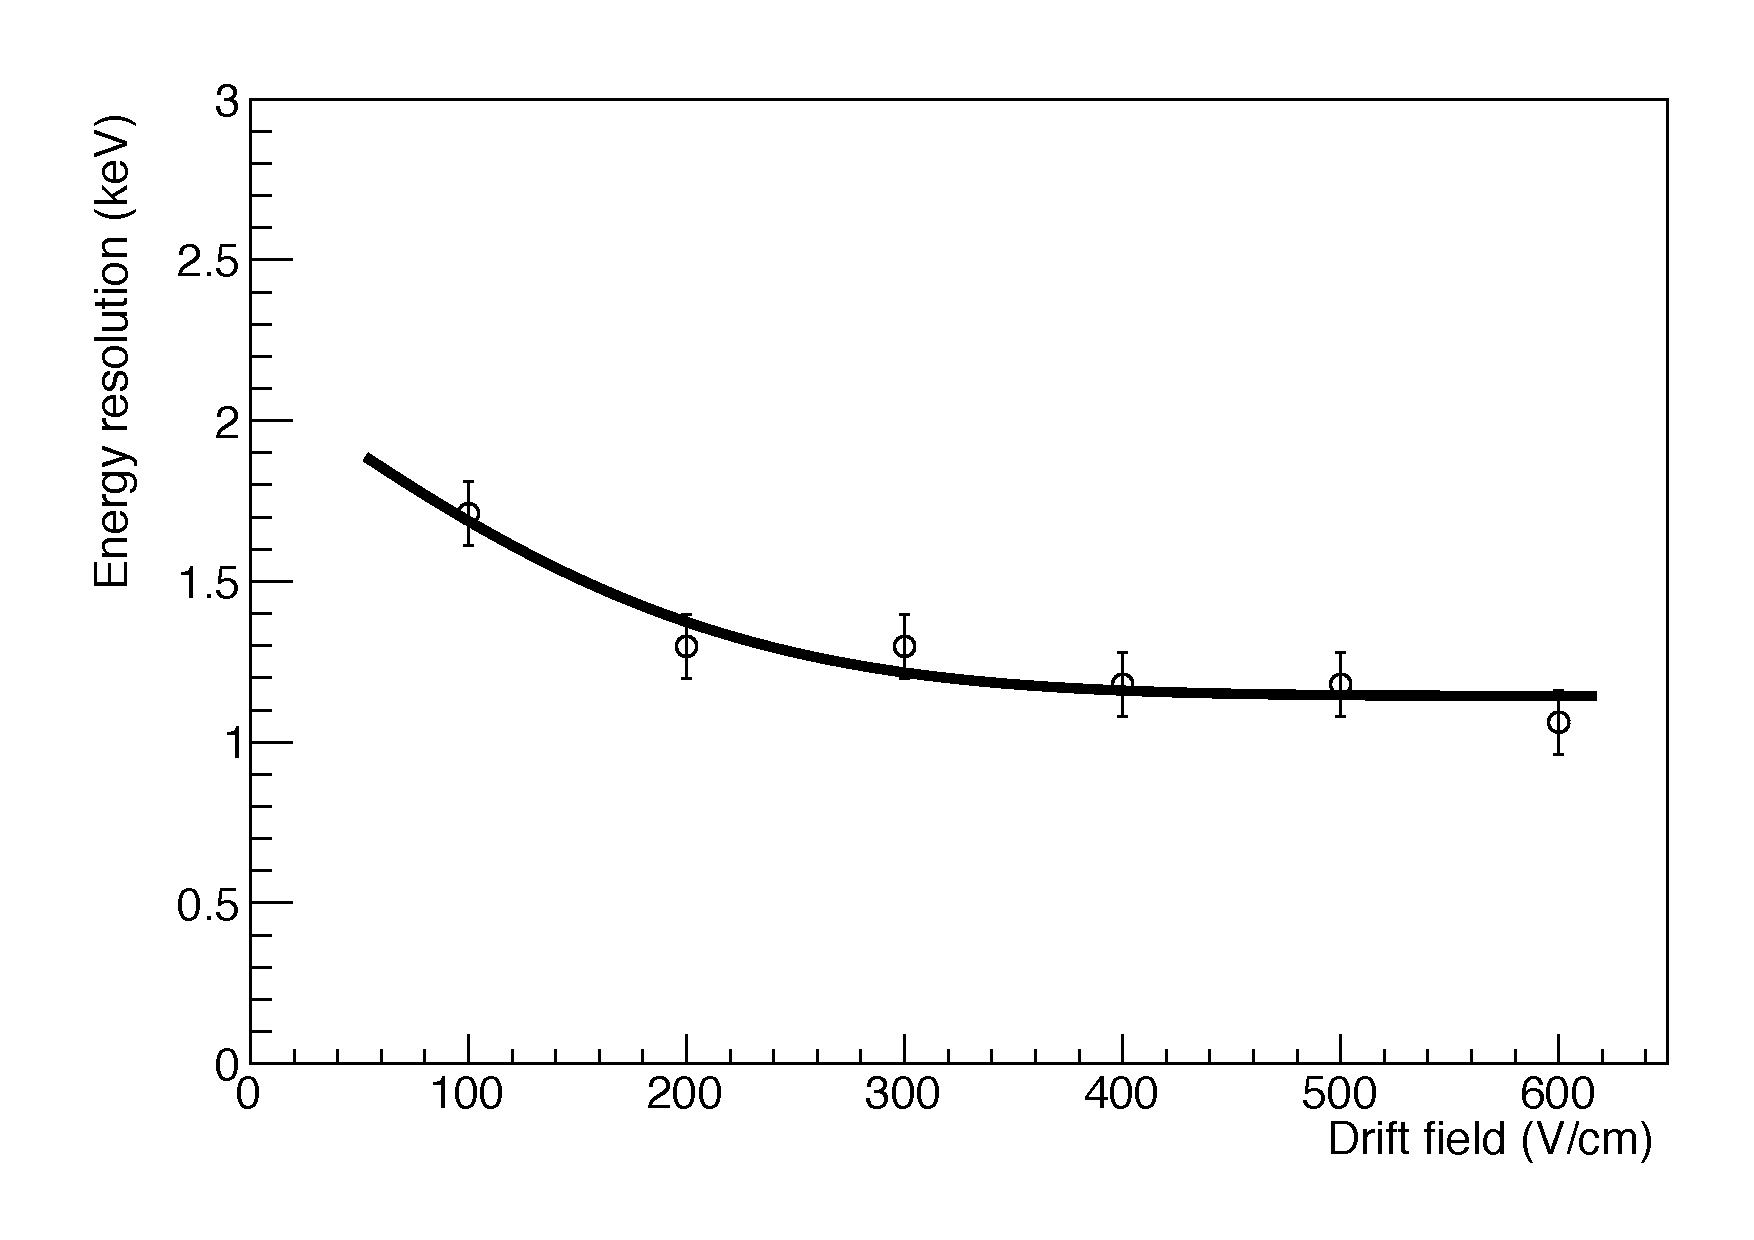
\includegraphics[width=.45\textwidth]{gEnergyRes_Edrift.pdf}
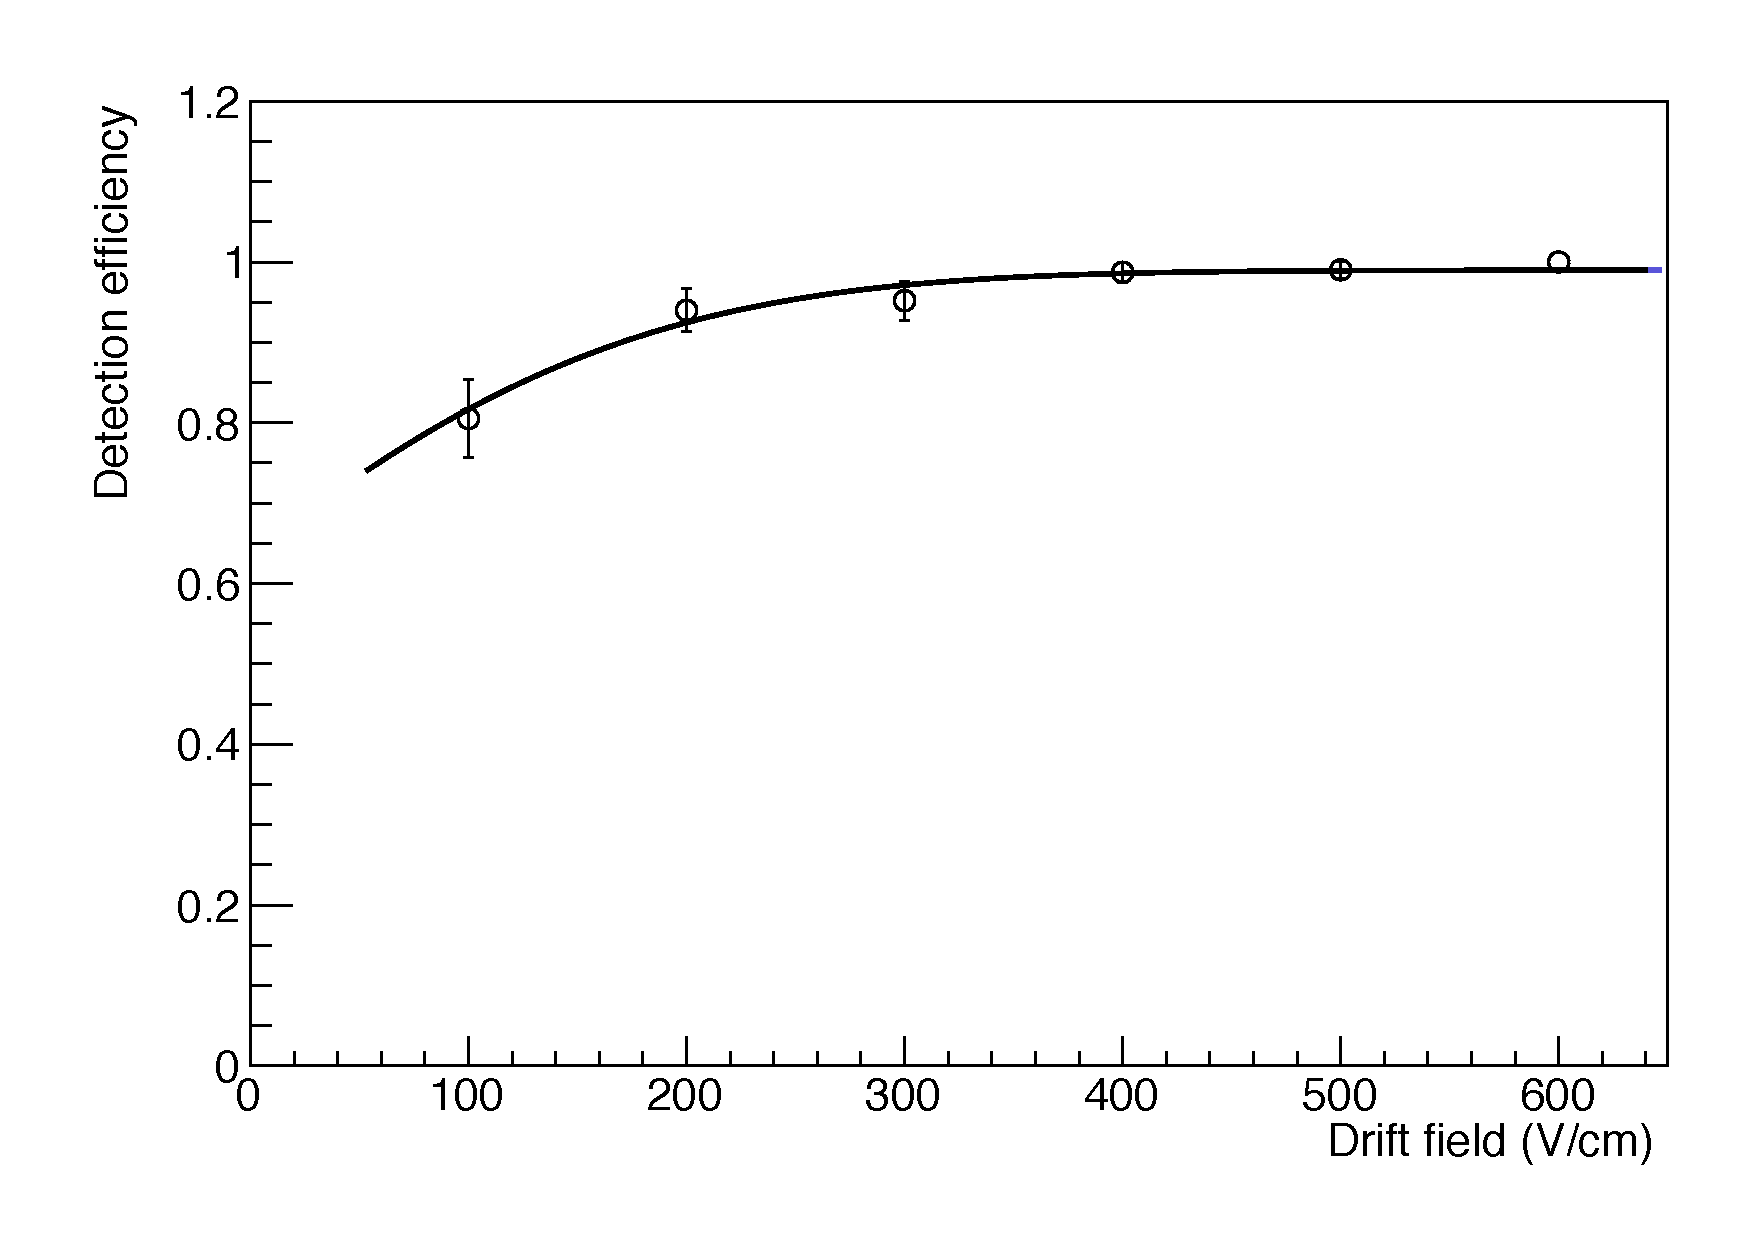
\includegraphics[width=.45\textwidth]{gEff_Edrift.pdf}
\caption{Left: average light spectrum (left) and  detection efficiency (right) as a function of E$_{\rm d}$ for a run taken with V$_{\rm GEM}$~=~450 V and E$_{\rm t}$ =~2 kV/cm.}
\label{fig:Ed1}
\end{figure}
Fluctuations of the number of photons per cluster (Fig. \ref{fig:Ed1},
left) have a small increase for small values of E$_{\rm d}$ (from
around 20\% to almost 30\%).  The detection efficiency
(Fig.~\ref{fig:Ed1} right) remains well above 95\% for E$_{\rm d}$
larger than 300 V/cm.

\item \textbf{Dependence on the Transfer Field (E$_{\rm t}$)}

The electric field in the gap between the GEM, E$_{\rm t}$, plays a
crucial role in the electron transport and on the effective gain of
the detector.  Because of a better capability in extracting electrons
\cite{bib:thesis}, the number of collected photons increases linearly
with the E$_{\rm t}$ reaching a value of 1200 for E$_{\rm t}$ = 2.5
kV/cm (while their fluctuations are quite stable around 20\%).  In
this configuration, therefore, a sensitivity of 0.2 collected photons
per released keV was measured.

\end{enumerate}

\section{Conclusion}

The analysis of the tests performed on the LEMON detector with the 5.9
keV photons provided an important characterisation of its
response. With a suitable field configuration (V$_{\rm GEM}$~=~460V,
E$_{\rm d}$~=~600~V/cm and E$_{\rm t}$~=~2.5 kV/cm), the response of
the detector is measured to be 1200 ph/cluster, i.e 1 photon each 5
released elettronvolts.  From the studies of the sensor intrinsic
noise, it was possible to determine that a threshold of 400 photons
ensures a rate of fake events smaller than 10 per year. With a
sensitivity of 0.2 ph/eV this would represent a threshold of 2 keV.
With an E$_{\rm t}$~=~2 kV/cm, the detection efficiency was estimated
to be well above 95\% down to V$_{\rm GEM}$~=~430 V where 1/3 of light
is collected compared to V$_{\rm GEM}$~=~460 V and E$_{\rm t}$~=~2.5
kV/cm.  Therefore, working with the latter settings would provide 3
more times light and thus, full detection efficiency seems possible
for 2 keV signals.

\bibliography{fe55}{}
\bibliographystyle{iopart-num}

\end{document}


